\documentclass[a4paper]{article}
 
% - taille de la fonte    : 10pt, 11pt, 12pt
% - recto ou recto-verso    : oneside, twoside
 
% Chargement d'extensions
%\usepackage[latin1]{inputenc}    
\usepackage[francais]{babel}    
\AtBeginDocument{\def\labelitemi{$\bullet$}}
%%%%%%%%%%%%%%%%%%%%%%%%%%%
\usepackage{amsthm}
\usepackage{amsmath}
\usepackage{amssymb}
\usepackage{mathrsfs}
\usepackage{graphicx}
\usepackage{geometry}
\usepackage{stmaryrd}
\usepackage{tikz}
\usetikzlibrary{patterns}

\usepackage[cache=false]{minted}
\usepackage{xcolor}
%\setbeamercolor{background canvas}{bg=lightgray}
\definecolor{LightGray}{gray}{0.9}
\definecolor{monOrange}{rgb}{0.97,0.35,0.04}

% Informations le titre, le(s) auteur(s), la date
\title{Vue3}
\author{Ibrahim ALAME}
\date{\today}
\includeonly{ introduction.tex} 
\begin{document}
 
\maketitle

\section{Objectifs du chapitre}
Ce chapitre va être une introduction approfondie au  {\color{monOrange}HTML}  . Nous allons voir toutes les bases du {\color{monOrange}HTML} dans ce chapitre : l'en-tête, les métadonnées les balises, les hyperliens, la structure des documents {\color{monOrange}HTML} etc.

Vous apprendrez entre autre à utiliser {\color{monOrange}Emmet} avec {\color{monOrange}Visual Studio Code}. Vous pouvez passer rapidement si vous connaissez déjà bien le langage mais un rafraîchissement ne peut pas vous faire de mal !

\section{Structure d'une page HTML}
\subsection{Création de notre première page HTML}
Créez un dossier pour notre cours où vous mettrez tous les projets que nous ferons ensemble : par exemple {\color{monOrange}dyma-htmlcss}.
\begin{enumerate}
\item Dans ce dossier créez un fichier {\color{monOrange}index.html}.
\item Ouvrez ensuite le dossier avec l'éditeur {\color{monOrange}VS Code} : soit en cliquant du droit sur le dossier, soit en ouvrant {\color{monOrange}VS code} et en allant dans {\color{monOrange}File > Open Folder}.
\end{enumerate}


Dans cette leçon, nous allons étudier la structure d'un document {\color{monOrange}HTML}.

Une page HTML minimale ressemble à cela :
\begin{minted}[
mathescape,
framesep=2mm,
baselinestretch=1.2,
%fontsize=\footnotesize,
bgcolor=LightGray,
%linenos
]{html}
<!DOCTYPE html>
<html>
  <head>
    <title>Le titre de ma page</title>
  </head>
  <body>
    <p>Le contenu de ma page</p>
  </body>
</html>
\end{minted}
Ce qui donne cela dans un navigateur :

\begin{center}
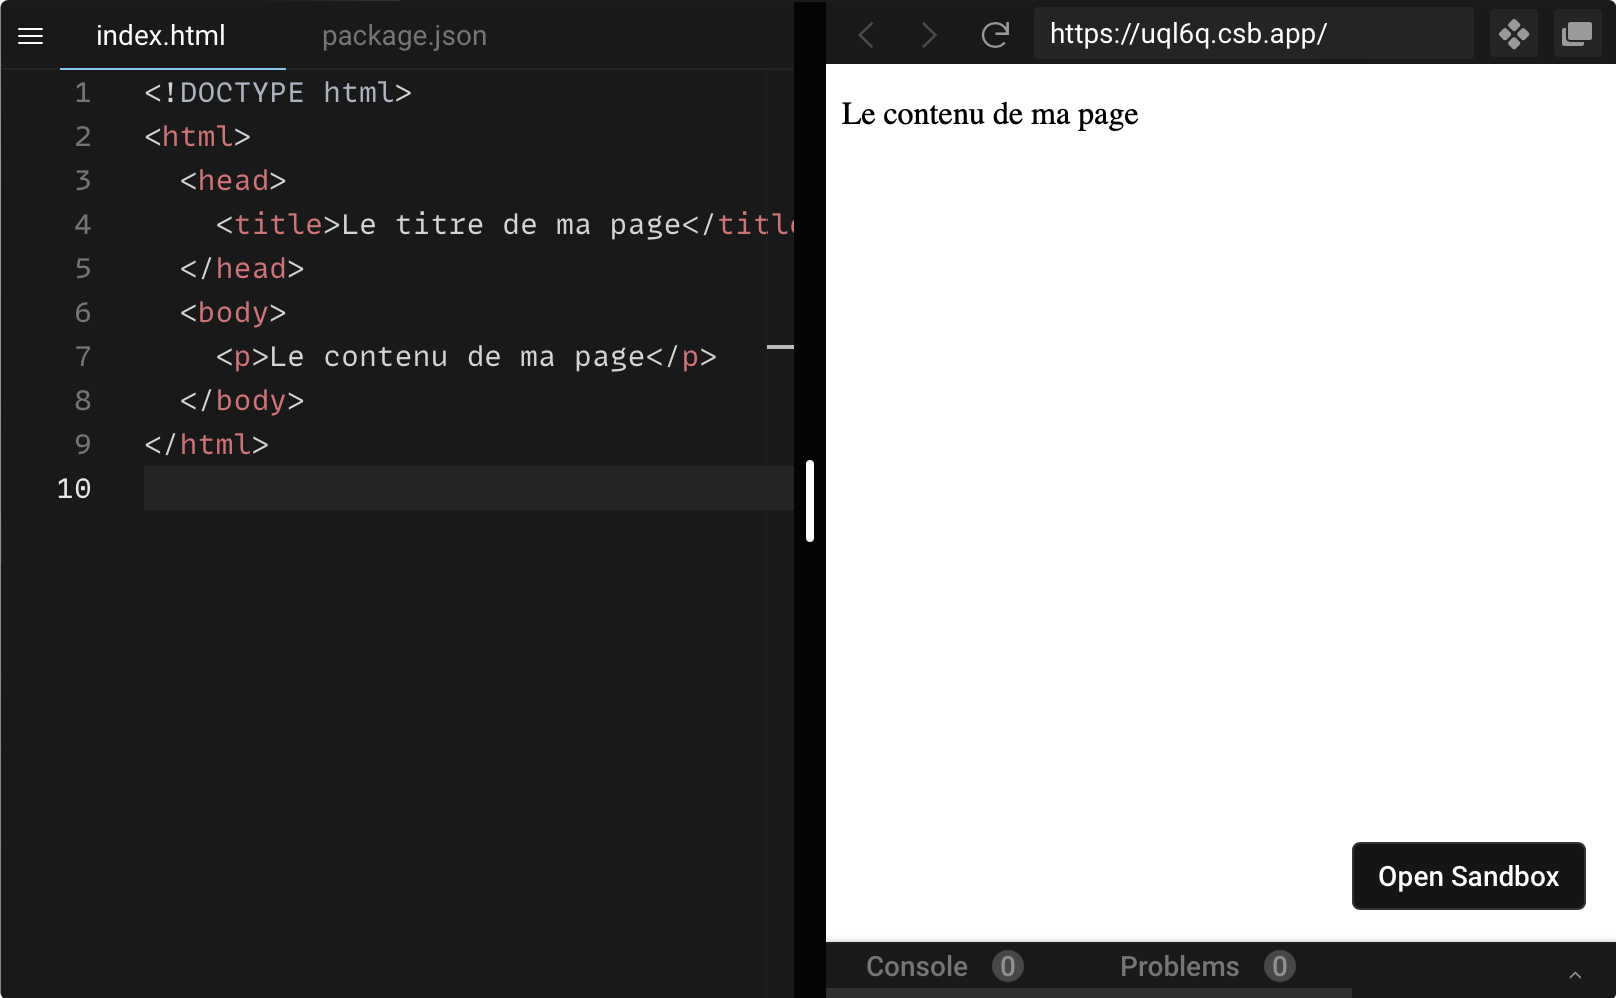
\includegraphics[width=10cm]{images/image01.png}
\end{center}

Nous allons utiliser à chaque fois un éditeur en ligne pour que vous puissiez exécuter directement le code. Mais nous vous invitons à le reproduire aussi sur votre ordinateur pour bien apprendre les notations en même temps. Nous allons d'abord voir ce que sont les balises en {\color{monOrange}HTML} puis nous étudierons la structure du document.

\subsection{Les éléments {\color{monOrange}HTML}}
Prenons un élément {\color{monOrange}HTML} par exemple :
\begin{minted}[
mathescape,
framesep=2mm,
baselinestretch=1.2,
%fontsize=\footnotesize,
bgcolor=LightGray,
%linenos
]{html}
<title>Le titre de ma page</title>
\end{minted}
\begin{itemize}
\item La première partie, {\tt <title>} , est une balise ouvrante. Il s'agit du nom de l'élément {\color{monOrange}HTML} ici {\color{monOrange}title} encadrés par des chevrons. Elle permet de déclarer le début de l'élément {\color{monOrange}HTML} ainsi que son type.

\item La deuxième partie est le contenu, ici {\color{monOrange}Le titre de ma page}, qui est simplement du texte dans notre cas.

\item La troisième partie, {\tt </title>}, est une balise fermante. Elle permet de déclarer la fin de l'élément {\color{monOrange}HTML}.
\end{itemize}


\subsection{L'imbrication}
Vous pouvez voir que les éléments {\color{monOrange}HTML} que nous avons déclarés s'imbriquent les uns dans les autres. Par exemple, {\tt <title>}, est imbriqué dans {\tt <head>}, lui-même imbriqué dans {\tt <html>}. Cette imbrication permet de créer la structure du document en déclarant quels éléments {\color{monOrange}HTML} sont inclus dans tels élément {\color{monOrange}HTML}.

\subsection{La structure d'une page {\color{monOrange}HTML}}
Nous allons maintenant étudier ligne par ligne la structure du document.

\subsubsection{Le type de document}
La première ligne d'un fichier{\color{monOrange} HTML} est la suivante :
\begin{minted}[
mathescape,
framesep=2mm,
baselinestretch=1.2,
%fontsize=\footnotesize,
bgcolor=LightGray,
%linenos
]{html}
<!DOCTYPE html>
\end{minted}
Il signifie au navigateur qu'il s'agit d'un document {\color{monOrange}HTML} à la version au moins 5. Comme nous l'avons vu, il n'y a plus aujourd'hui de version {\color{monOrange}HTML}, il existe uniquement un {\color{monOrange}HTML Living Standard} qui évolue constamment. Cette ligne, et l'extension {\color{monOrange}.html} du fichier, permettent également aux éditeurs de pouvoir parser le document pour mettre les couleurs et activer l'autocomplétion {\color{monOrange}HTML}.

\subsubsection{L'élément racine {\color{monOrange}html}}
La deuxième ligne est une balise ouvrante {\tt <html>}. L'élément {\tt <html>} contient tout le code de la page et est appelé élément racine.

\subsubsection{L'en-tête {\color{monOrange}head}}
L'élément {\color{monOrange}HTML head} est l'en-tête du document. Il ne peut y en avoir qu'un par page. Il contient les éléments que vous voulez inclure dans la page {\color{monOrange}HTML} sans qu'ils soient affichés aux utilisateurs. Il peut contenir de nombreux éléments que nous verrons au fur et à mesure. Il contient notamment le titre de la page.

\subsubsection{Le titre de la page {\color{monOrange}title}}
L'élément {\color{monOrange}title} permet de déclarer le titre de la page dans l'en-tête {\color{monOrange}head}. Il s'affiche dans l'onglet du navigateur. Il est également utilisé comme description de la page pour l'ajout en favori dans le navigateur.

\subsubsection{le corps {\color{monOrange}body}}
L'élément {\color{monOrange}body} contient tout le contenu à afficher aux utilisateurs de votre page. Il contiendra le texte, les éventuelles images, vidéos, musiques etc.

\subsection{Utilisation des extensions {\color{monOrange}Prettier} et {\color{monOrange}Emmet}}
Nous allons commencer à utiliser deux extensions dans {\color{monOrange}VS Code}.

\subsubsection{{\color{monOrange}Emmet}}
Cette extension est incluse dans {\color{monOrange}VS code} par défaut. Elle permet d'utiliser des raccourcis extrêmement utiles pour la génération de code {\color{monOrange}HTML} et {\color{monOrange}CSS}.

Nous allons l'utiliser tout le temps dans la formation et vous expliquerons à chaque fois comment gagner du temps en vous donnant les syntaxes appropriées.

\subsubsection{{\color{monOrange}Prettier}}
{\color{monOrange}Prettier} permet de mettre en forme le code automatiquement lorsque vous le sauvegardez. C'est une extension très utile et nous vous invitons à l'installer dans VS code;
\begin{enumerate}
\item Allez dans {\color{monOrange}Extensions} puis recherchez {\color{monOrange}Prettier}. Ensuite cliquez sur {\color{monOrange}Install}. {\color{monOrange}Prettier} a plus de 14 millions de téléchargement sur VS code ce qui en fait l'une des extensions les plus utilisées.

\item Dans {\color{monOrange}VS Code} allez ensuite dans {\color{monOrange}File} puis {\color{monOrange}Preferences} puis {\color{monOrange}Settings}. Recherchez {\color{monOrange}format on save} et cochez la case.

\item Toujours dans {\color{monOrange}VS Code}, et toujours dans {\color{monOrange}Settings}. Recherchez cette fois {\color{monOrange}Default Formatter} et dans la liste déroulante sélectionnez {\color{monOrange}Prettier - Code Formatter esbenp.prettier-vscode}.

\end{enumerate}
{\color{monOrange}Prettier} fonctionnera maintenant à chaque fois que vous sauvegardez !



\subsection{Affichage d'une page HTML}
\subsubsection{Ouvrir un document {\color{monOrange}HTML} local dans le navigateur}
Vous pouvez afficher un document {\color{monOrange}HTML} à l'aide de n'importe quel navigateur. 
\begin{itemize}
\item Bien qu'il existe plus de 100 navigateurs différents, les plus performants sont actuellement probablement Chrome, Firefox et Brave.

\item Dans la formation nous utiliserons Chrome, mais Firefox et Brave sont également très biens.

\item Pour ouvrir un fichier {\color{monOrange}.html} avec un navigateur, cliquez droit et faites ouvrir avec {\color{monOrange}Chrome} par exemple. Ou ouvrir avec une autre application et sélectionnez un navigateur.
\end{itemize}

Vous aurez ensuite :

\begin{center}
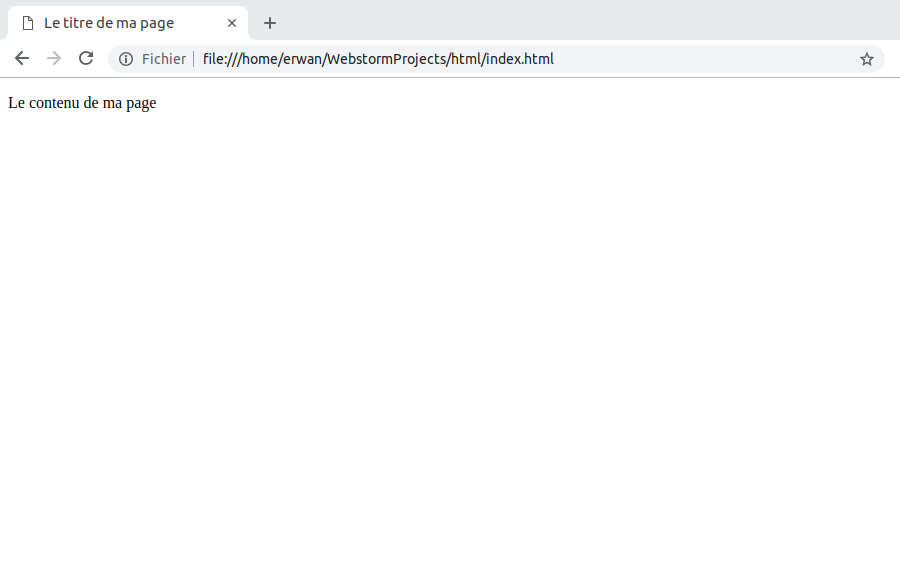
\includegraphics[width=10cm]{images/image02.png}
\end{center}

\subsubsection{Ouvrir un document {\color{monOrange}HTML} depuis le {\color{monOrange}Web}}
Lorsque vous ouvrez une page {\color{monOrange}HTML} en utilisant le {\color{monOrange}Web} et {\color{monOrange}Internet}, votre navigateur va envoyer une requête HTTP à l'adresse demandée, par exemple {\color{monOrange}https://fr.wikipedia.org/}. Les serveurs {\color{monOrange}Web} de {\color{monOrange}Wikipedia} vont alors traiter la requête et retourner une réponse {\color{monOrange}HTTP} que votre navigateur interprétera pour afficher la page. Par exemple :
\begin{center}

\includegraphics[width=10cm]{images/image03.png}
\end{center}

\subsubsection{Ouvrir un document {\color{monOrange}HTML} local en utilisant un serveur local}
Il existe un inconvénient à ouvrir un fichier {\color{monOrange}HTML} directement dans votre navigateur : les changements ne sont pas pris en compte. Autrement dit, lorsque vous effectuez des modifications dans {\color{monOrange}VS code} du fichier {\color{monOrange}HTML} et que vous sauvegardez (avec {\color{monOrange}Ctrl + s}), la page affichée dans le navigateur ne se met pas automatiquement à jour. Il faut nécessairement rafraichir la page dans le navigateur pour voir les changements.

Il existe heureusement une solution : utiliser un serveur {\color{monOrange}Web} local qui va suivre les changements effectués dans votre fichier et mettre automatiquement la page à jour. Pour cela, allez dans {\color{monOrange}VS code}, puis dans {\color{monOrange}Extensions} puis recherchez {\color{monOrange}Liver server} et installez la.

Cette extension permet de lancer un serveur sur {\color{monOrange}127.0.0.1} qui est une adresse {\color{monOrange}IP} spéciale faisant référence à votre ordinateur. La requête n'ira ainsi pas sur {\color{monOrange}Internet} et vous n'avez pas besoin de connaître l'adresse {\color{monOrange}IP} réelle de votre ordinateur. Cette adresse {\color{monOrange}IP} a un alias, c'est-à-dire un nom de domaine qui y équivaut, {\color{monOrange}localhost}. Tapez {\color{monOrange}localhost} ou {\color{monOrange}127.0.0.1} est donc équivalent.

{\color{monOrange}Live server} permet de lancer un serveur de développement local qui a permet automatiquement de mettre à jour la page en cas de changement dans le code (c'est ce qu'on appelle le {\color{monOrange}live reload}). Pour lancer une page {\color{monOrange}HTML} avec l'extension vous pouvez soit cliquer droit dans le fichier dans l'éditeur et faire {\color{monOrange}Open with Live Server}. Vous pouvez également cliquer sur {\color{monOrange}Go Live} en bas à droite. Vous pouvez enfin utiliser le raccourci : {\color{monOrange}Alt +L} puis {\color{monOrange}Alt + O}.

Voici un exemple :

\begin{center}
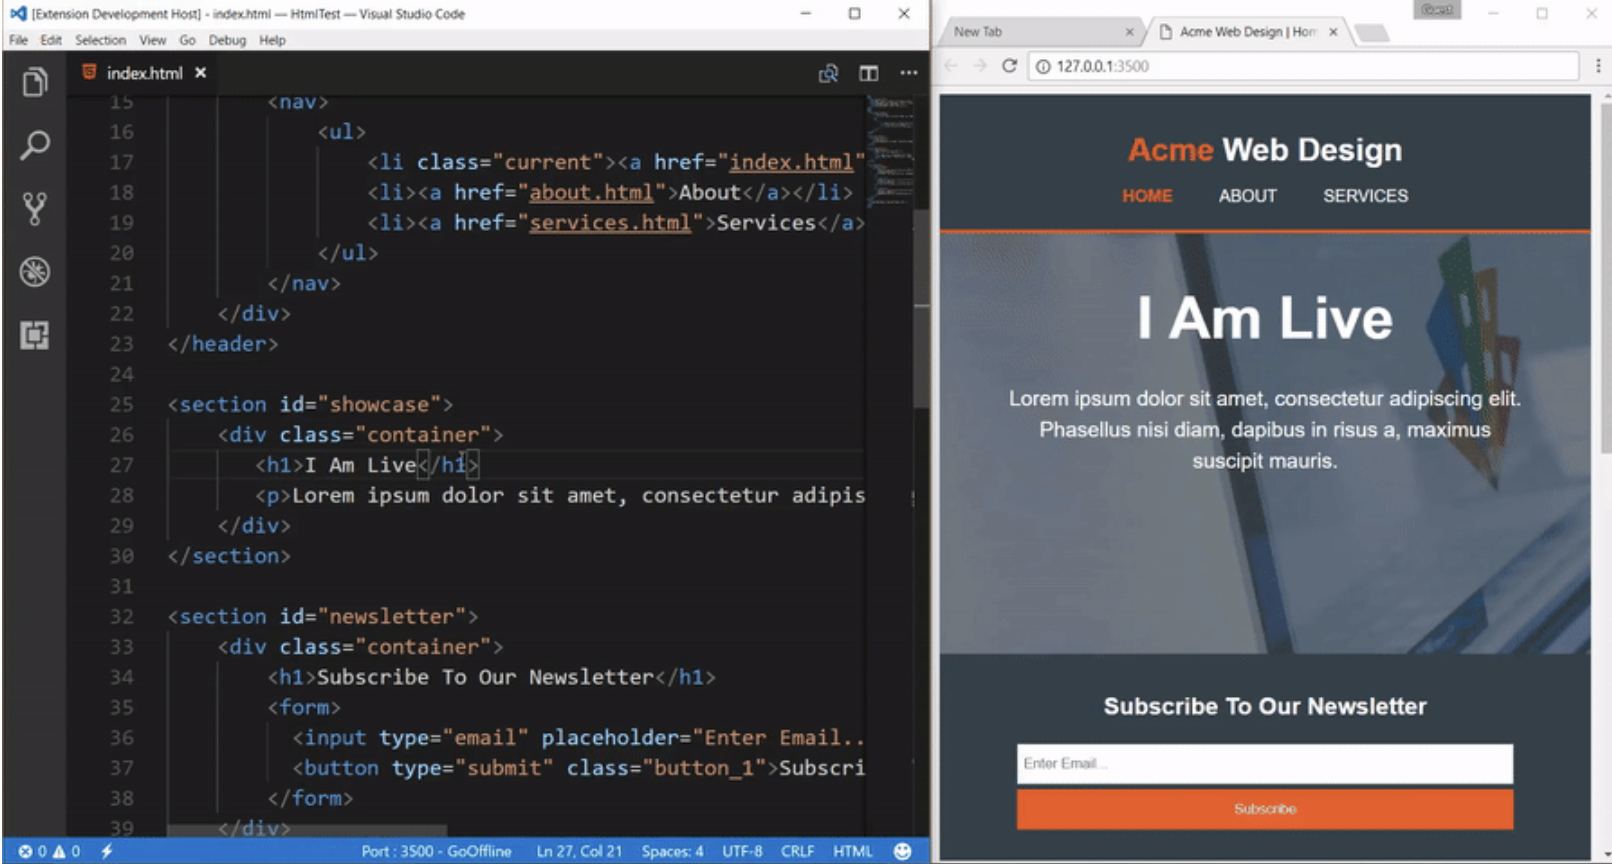
\includegraphics[width=10cm]{images/image04.png}
\end{center}

%%%%%%%%%%%%%%%%%%%%%%%%%%%%%%%%%%%%%%%%%%%%%%%%%%%%%%%%%%%%%%%%%%%%%%%%%%%%%%%%%%%%

\section{Les attributs HTML et les métadonnées}
\subsection{Génération d'un document {\color{monOrange}HTML} avec Emmet}
\begin{enumerate}
\item Nous allons commencer par générer un document {\color{monOrange}HTML} avec {\color{monOrange}Emmet}.

\item Supprimez ce que vous aviez dans index.html.

\item Entrez ensuite :
\begin{minted}[
mathescape,
framesep=2mm,
baselinestretch=1.2,
%fontsize=\footnotesize,
bgcolor=LightGray,
%linenos
]{html}
!
\end{minted}

Vous aurez une autocomplétion : 
\begin{center}
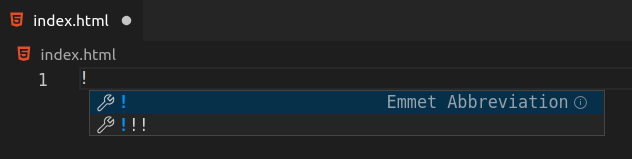
\includegraphics[width=10cm]{images/image05.png}
\end{center}

Vous pouvez alors presser la touche entrée et obtiendrez le document suivant :
\begin{minted}[
mathescape,
framesep=2mm,
baselinestretch=1.2,
%fontsize=\footnotesize,
bgcolor=LightGray,
%linenos
]{html}
<!DOCTYPE html>
<html lang="en">
  <head>
    <meta charset="UTF-8" />
    <meta name="viewport" content="width=device-width, initial-scale=1.0" />
    <meta http-equiv="X-UA-Compatible" content="ie=edge" />
    <title>Document</title>
  </head>
  <body></body>
</html>
\end{minted}


\end{enumerate}
\begin{itemize}
\item Si vous n'avez pas de suggestion qui apparait, vous pouvez presser les touches {\color{monOrange}Ctrl + Espace}.

\item Si ce raccourci ne se déclenche pas sur un Tab allez dans Fichier > Préférences > Paramètres et recherchez {\color{monOrange}Emmet}. Cochez la case {\color{monOrange}Emmet: Trigger Expansion On Tab}.

\end{itemize}
\subsection{Les attributs}
Les éléments {\color{monOrange}HTML} peuvent avoir des attributs. Un attribut est par exemple {\color{monOrange}lang }:
\begin{minted}[
mathescape,
framesep=2mm,
baselinestretch=1.2,
%fontsize=\footnotesize,
bgcolor=LightGray,
%linenos
]{html}
<html lang="fr">
\end{minted}
Les attributs contiennent des informations supplémentaires sur l'élément {\color{monOrange}HTML}  sans qu'elles n'apparaissent directement sur la page. Pour créer un attribut il y a trois règles :
\begin{enumerate}
\item  Il faut mettre un espace entre le nom de l'élément {\color{monOrange}HTML}  dans la balise ouvrante, et le nom de l'attribut, ou entre l'attribut précédent si il y a plusieurs attributs.

\item  Il faut donner un nom à l'attribut et ajouter le signe égal.

\item   Il faut donner une valeur à l'attribut. Il faut la placer à l'intérieur de guillemets, qui peuvent être simples ou doubles dès lors que la valeur contient un des caractères suivants {\tt " ' ` = < >}. Cependant, vous trouverez quasiment systématiquement des guillemets autour de la valeur et nous vous invitons donc à toujours en mettre.
\end{enumerate}

Parfois, il est possible d'utiliser une notation raccourcie avec les attributs booléens :

\begin{minted}[
mathescape,
framesep=2mm,
baselinestretch=1.2,
%fontsize=\footnotesize,
bgcolor=LightGray,
%linenos
]{html}
<input type="text" disabled>
\end{minted}
Ces attributs ne peuvent avoir qu'une seule valeur qui est la plupart du temps le nom de l'attribut.

\subsubsection{L'attribut {\color{monOrange}lang}}
Dans le document généré par {\color{monOrange}Emmet}, nous utilisons donc l'attribut {\color{monOrange}lang} sur l'élément {\color{monOrange}html}. Cet attribut permet de définir la langue principale du document. Par défaut, il est défini à {\color{monOrange}en} pour {\color{monOrange}english} mais mettez {\color{monOrange}fr} pour une page en français. La langue est utilisée pour l'indexation par les moteurs de recherche.

\subsection{Les métadonnées}
Les métadonnées sont des données apportant des informations sur d'autres données. Le langage {\color{monOrange}HTML} permet d'utiliser des métadonnées dans un document en utilisant la balise {\color{monOrange}meta}.

\subsubsection{Le {\color{monOrange}charset}}
La métadonnée permet de définir l'encodage des caractères du document. C'est le jeu de caractères à utiliser pour convertir les valeurs numériques en caractères. Ici, nous utilisons {\color{monOrange}UTF-8} qui permet d'encoder n'importe quel caractère (latin, japonais, chinois, caractères spéciaux). C'est l'encodage le plus utilisé sur le {\color{monOrange}Web}, et plus de 95% des sites l'utilise.

\subsubsection{Le {\color{monOrange}viewport}}
Le {\color{monOrange}viewport} est la surface de la fenêtre du navigateur. Nous allons étudier ce que veut dire cette balise {\color{monOrange}meta} :

\begin{minted}[
mathescape,
framesep=2mm,
baselinestretch=1.2,
%fontsize=\footnotesize,
bgcolor=LightGray,
%linenos
]{html}
<meta name="viewport" content="width=device-width, initial-scale=1.0" />
\end{minted}

Elle est utile pour l'affichage sur les mobiles et les tablettes. Pour bien comprendre il faut déjà voir les deux surfaces existantes pour les appareils mobiles et tablettes.
\begin{itemize}
\item La première est la surface physique qui est le nombre de pixels sur l'écran, qui est également appelée la définition de l'écran.
\item La deuxième est la surface utilisable qui est le nombre de pixels virtuels que le terminal pense pouvoir afficher.
\end{itemize}

Ces surfaces ne sont pas égales sur les mobiles pour des raisons d'affichage. La taille du viewport d'un mobile n'est ni égale à sa surface physique, ni égale à sa surface virtuelle, et ce pour pouvoir afficher la plupart des pages Web. Elle est supérieure afin de pouvoir appliquer un dézoom de la page pour l'afficher en entier. Sans la balise viewport, le navigateur mobile réagit comme sur un ordinateur et met la page à l'échelle de l'écran, ce qui rend impossible la lecture du contenu. Sans la balise nous aurions l'affichage de gauche, et avec la balise l'affichage de droite :
\begin{center}
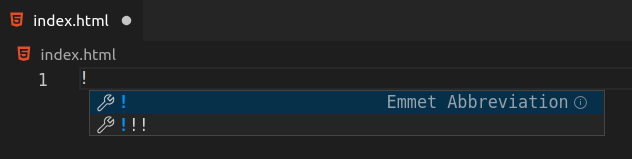
\includegraphics[width=10cm]{images/image05.png}
\end{center}

La balise {\color{monOrange}viewport} permet donc d'indiquer au navigateur mobile comment ajuster les dimensions et l'échelle de la page à la largeur de l'appareil.
\begin{itemize}
\item {\tt width="device-width"} permet de définir la largeur de la fenêtre du viewport à celle de l'appareil.

\item {\tt initial-scale="1.0} permet de définir le niveau de zoom initial.
\end{itemize}


Autrement dit, ces deux paramètres permettent de forcer l'appareil mobile à ne pas changer le zoom ou prétendre que la largeur disponible est plus importante que réellement pour tenter d'afficher l'intégralité de la page. Il nous permettra plus tard dans la formation d'adapter notre page et nos styles en fonction de la largeur réelle disponible et donc de créer un site {\color{monOrange}responsive} comme sur l'image à droite.

\subsection{La {\color{monOrange}meta X-UA-Compatible}}
Ce tag permet d'empêcher le mode compatibilité sur {\color{monOrange}Internet Explorer} et de forcer le navigateur à utiliser le dernier moteur de rendu disponible (dernière version du moteur {\color{monOrange}Edge}). Ce {\color{monOrange}tag} n'est pas utile si vous ne souhaitez pas supporter Internet Explorer qui représente moins de 1\% du marché des navigateurs.

\subsubsection{La {\color{monOrange}meta description}}
La {\color{monOrange}meta} description sert à l'indexation de cette page par les moteurs de recherche et les annuaires. Elle doit contenir une description du contenu de la page en une ou deux phrases. Depuis 2017, Google affiche entre 260 et 300 caractères. Il faut donc adapter la description en conséquence. Elle s'utilise de cette manière :
\begin{minted}[
mathescape,
framesep=2mm,
baselinestretch=1.2,
%fontsize=\footnotesize,
bgcolor=LightGray,
%linenos
]{html}
<meta name="description" content="La description de la page." />
\end{minted}









\end{document}
